%!TEX root = thesis.tex

\chapter{Visualisation Refinement}
\label{chap:visualisation-refinement}

Following the first user study (Chapter~\ref{chap:user-study}), limitations with both the visualisations and the evaluation method were identified and steps were taken to correct the limitations. The following sections seek to identify the limitations and the steps taken.

\section{Rationale}



\section{Design}

\begin{figure}
  \centering 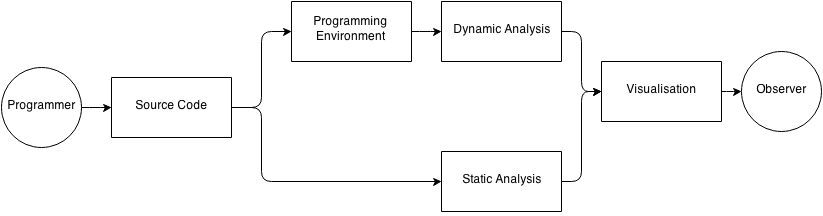
\includegraphics[width=\columnwidth]{../images/diagrams/knowledge-flow}
  \caption{Knowledge flow from programmer to observer as directed by the visualisation technique employed.}
\label{fig:knowledge-flow}
\end{figure}

\begin{figure}
  \centering 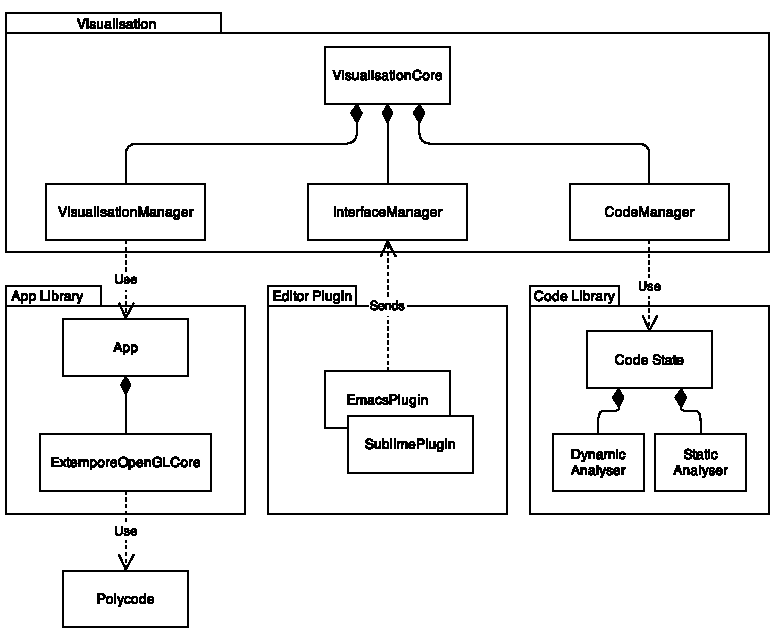
\includegraphics[width=\columnwidth]{../images/diagrams/visualisation-class-diagram}
  \caption{Class diagram of the visualisation technique employed.}
\label{fig:visualisation-class-diagram}
\end{figure}

\section{Analysis}

Both dynamic program analysis and static source code analysis have been used to implement the visualisations (see combined static and dynamic approach taken in \cite{Eisenbarth2003}).

\section{Mappings}

A number of specific mappings were assigned to the visualisation. These visual mappings related directly to actions taken by the programmer. 

% See Table~\ref{} for a listing of these mappings.

